\section{Clustering}
An iterative process was employed to evaluate various feature configurations for clustering. Each configuration involved outlier detection, clustering, and subsequent analysis to interpret and characterize the resulting clusters. This approach enabled the identification of the most meaningful features to optimize clustering performance.
After several iterations, the three key features selected were: \textit{avg\_relative\_position}, \textit{mean\_sq}, and \textit{career\_level}. Using these features, our goal was to achieve a clustering that would allow us to identify groups of cyclists based on their cycling performance, considering how well a cyclist has positioned himself, how much he has competed in his career, and how important the races he has competed in have been. 
To obtain comparable results, we used the same three features with all clustering algorithms finding out that K-Means delivered the best results according to our characterization goal.
In the following sections, we provide an overview of the entire process.

\subsection{Outlier Detection}
Outlier detection was essential to ensure that extreme values or outliers did not significantly affect the clustering results, allowing more accurate and meaningful groupings. Three different techniques were employed:
\begin{itemize}
    \vspace{-0.20cm}
    \item \textbf{One-class SVM}: it identified 120 outliers
    \vspace{-0.20cm}
    \item \textbf{Connectivity Approach}: it identified 107 outliers 
    \vspace{-0.20cm}
    \item \textbf{Isolation Forest}: it identified 89 outliers
\end{itemize}
\vspace{-0.20cm}

\noindent
Finally, we implemented a customized strategy by combining the results of these methods in an ensemble fashion. Specifically, we adopted a majority voting approach: rows identified as outliers by at least two methods were excluded from the dataset. Through this approach, 70 outliers were identified, and removed; results are shown in \autoref{fig:outlier}.

\begin{figure}[H]
\centering
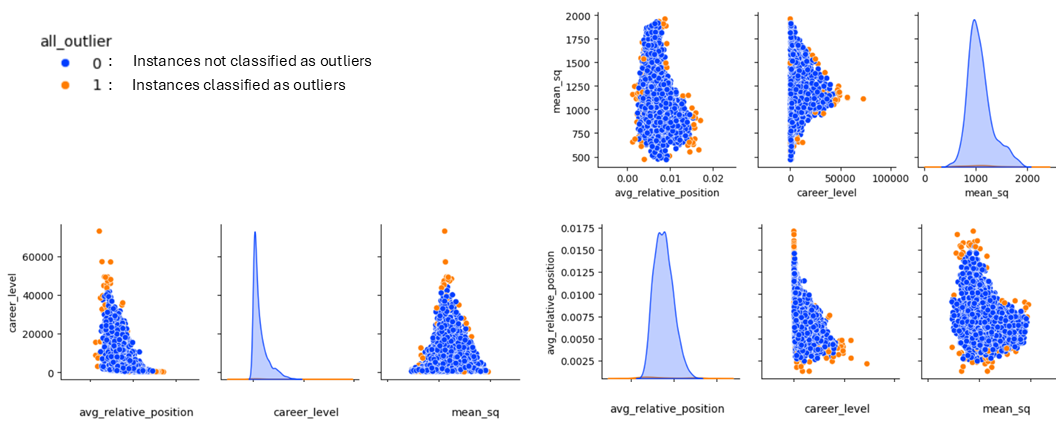
\includegraphics[width=0.9\textwidth]{images/CLUSTER/outlier.png}
\caption{ \small Outliers identified using majority voting ensemble approach\small }
\label{fig:outlier}
\end{figure}


%---------------------------------------------------------
\subsection{K-means Clustering}
\subsubsection{Preprocessing, Best K, and Visualization}

Initially, all the selected features were scaled to have zero mean and unitary standard deviation. This preprocessing step is essential as it improves the performance of the K-means algorithm, which is sensitive to the scale of the input features. \\

\noindent
\textbf{Best K Parameter Search}\\
A grid search was conducted to test different configurations of the parameter k (number of clusters). For each configuration, we plotted the SSE, Silhouette, and Davies-Bouldin scores to monitor clustering performance. While these plots provided valuable insights, the final choice of k was not only based on them.
Since clustering is an exploratory process and good metric scores do not always guarantee that clusters align with our expectations or domain-specific needs, we also performed cluster characterization for various k values to evaluate different results more empirically.
Therefore, the decision for the optimal k was made by combining the analysis of the metrics in \autoref{fig:metrics_kmeans} with the evaluation of the characterization and significance of the clusters finding \textbf{k=3} as best k.\\

\begin{figure}[H]
    \centering
    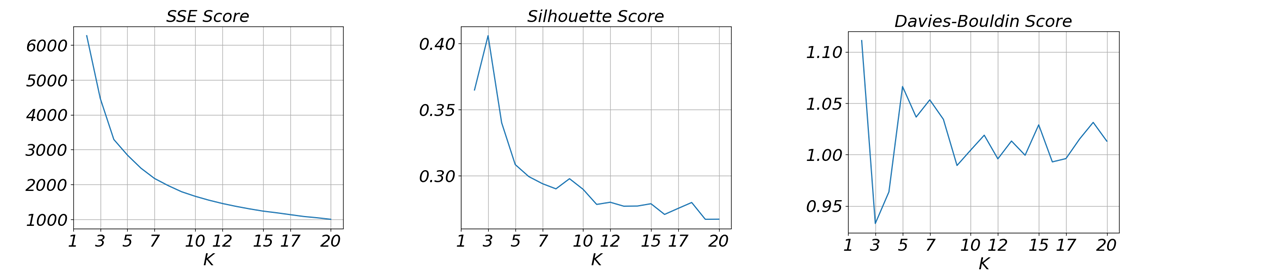
\includegraphics[width=1\textwidth]{images/CLUSTER/k-means/metrics.png}
    \caption{ \small Trends of K-means SSE, Silhouette, and Davies-Bouldin scores as the number of clusters \( k \) increases.}
    \label{fig:metrics_kmeans}
\end{figure}

\noindent
\textbf{Visualization Analysis}\\
From the pair plot and PCA plot in \autoref{fig:pairplot_kmeans}, one can observe that clusters are generally well separated. However, some overlaps are visible indicating that while the clustering captures the overall structure of the data effectively, some degree of variability or noise remains. These overlaps suggest that the boundaries between clusters are not entirely rigid, likely reflecting the inherent complexity or overlapping characteristics of the dataset.

\begin{figure}[H]
\centering
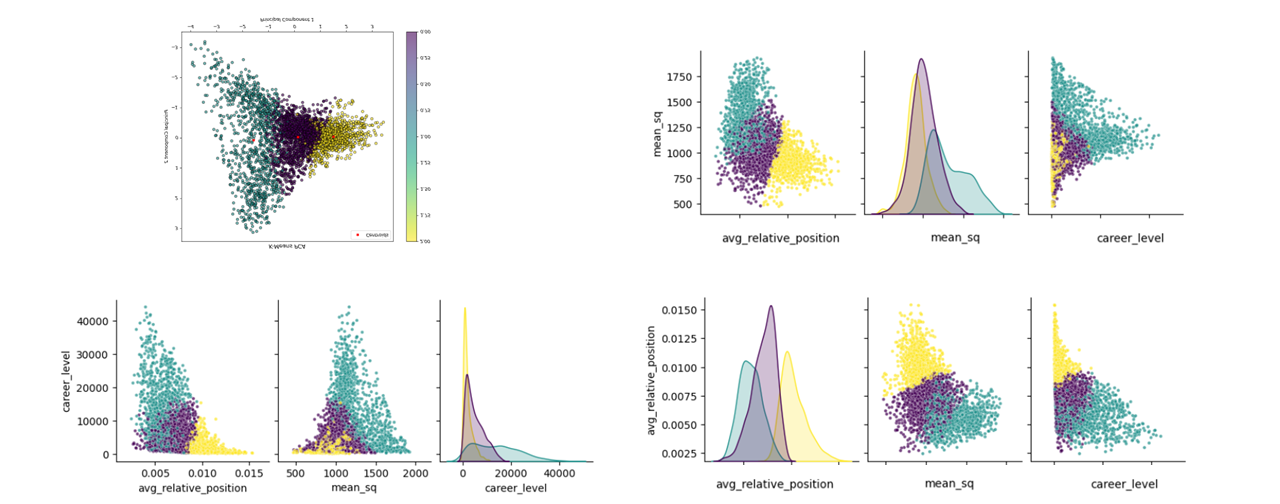
\includegraphics[width=0.9\textwidth]{images/CLUSTER/k-means/pairplot.png}
\caption{ \small K-means feature pair plots and PCA visualization \small }
\label{fig:pairplot_kmeans}
\end{figure}

\subsubsection{Characterization}
Starting by examining the Parallel Coordinates Plot for Centroids in \autoref{fig:cluster_centroids}, we have an overview of the identified clusters that are characterized as follows:

\vspace{-0.2cm}

\begin{itemize}
    \item \textbf{Cluster 0}: \textit{Intermediate Cyclists}
    \vspace{-0.2cm}
    \item \textbf{Cluster 1}: \textit{Best Cyclists}
    \vspace{-0.2cm}
    \item \textbf{Cluster 2}: \textit{Worst Cyclists}
\end{itemize}

\vspace{-0.2cm}


\begin{figure}[H]
\centering
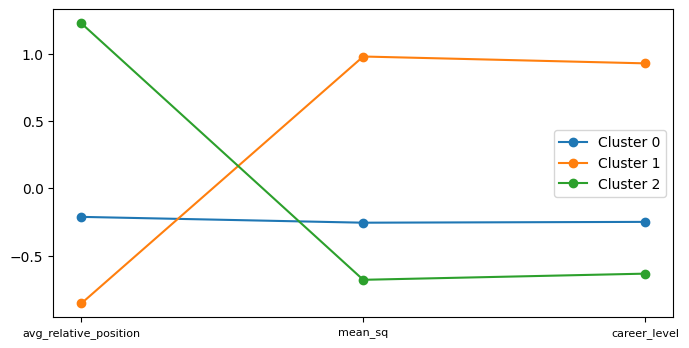
\includegraphics[width=0.5\textwidth]{images/CLUSTER/k-means/Centroids_plot.png}
\caption{ \small \small K-means Parallel Coordinates Plot for Centroids}
\label{fig:cluster_centroids}
\end{figure}

\noindent
The cyclists in the \textit{Best Cyclists} cluster have a low average relative position (meaning they often finish among the top), high average start list quality, and a high career level. In contrast, cyclists in the \textit{Worst Cyclists} cluster show the opposite values. Those in the \textit{Intermediate Cyclists} cluster fall somewhere in between.
Further analysis of the mean values of each feature across clusters aligns with the patterns observed in the \autoref{fig:cluster_centroids}, confirming consistent trends for features such as career level, mean start list quality, and average relative position.\\

\noindent
\textbf{Insights from Non-Clustering Features}

\noindent
We then analyzed the distributions of additional features that were not directly used with the clustering algorithms but provided valuable insights into cyclist's quality and experience. Examining these distributions ensures that the clusters are accurately interpreted and align with the expected performance levels that emerged during the characterization process.

%---- WEIGHTED PODIUMS
The distribution of \textbf{weighted podiums} reveals distinct patterns across the clusters. In the first plot of \autoref{fig:podiums_distr_kmenas}, a significant proportion of cyclists have a weighted podium count of 0, with a sharp decline as the count increases slightly. Conversely, in the second and third plots, corresponding to higher-ranked cyclists, the decline is more gradual. This trend illustrates the superior ability of cyclists in these clusters to consistently achieve higher placements.  

\begin{figure}[H]  
\centering  
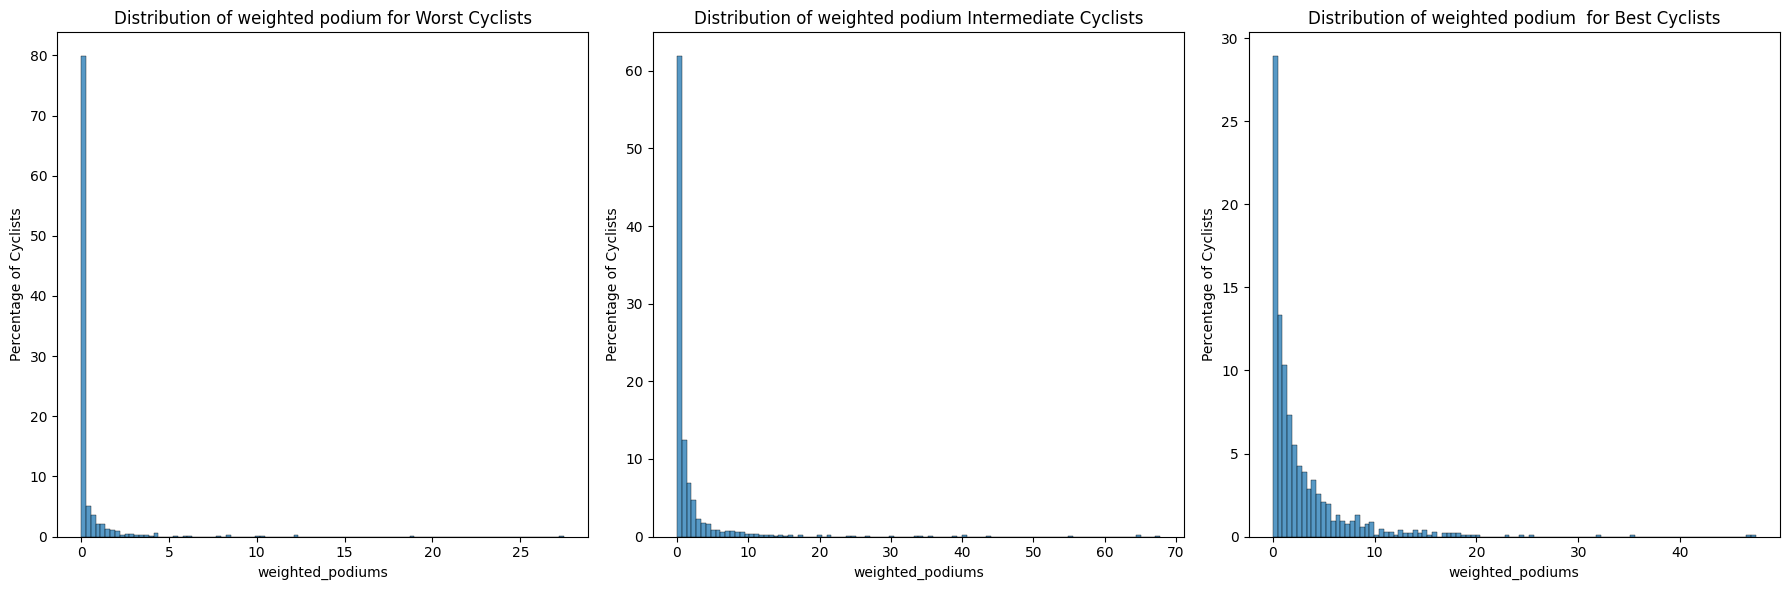
\includegraphics[width=0.93\textwidth]{images/CLUSTER/k-means/podiums_distr.png}  
\caption{ \small K-means weighted podiums distribution, with cyclists represented as percentage}  
\label{fig:podiums_distr_kmenas}  
\end{figure}  

\noindent  
\textbf{Cyclist experience} also demonstrates an expected progression across clusters. As shown in \autoref{fig:experience_distr_kmenas}, the percentage of highly experienced cyclists rises as we move from the worst-performing cluster to the best-performing one. This pattern aligns with expectations, reinforcing the notion that experience correlates with superior performance.  

\begin{figure}[H]  
\centering  
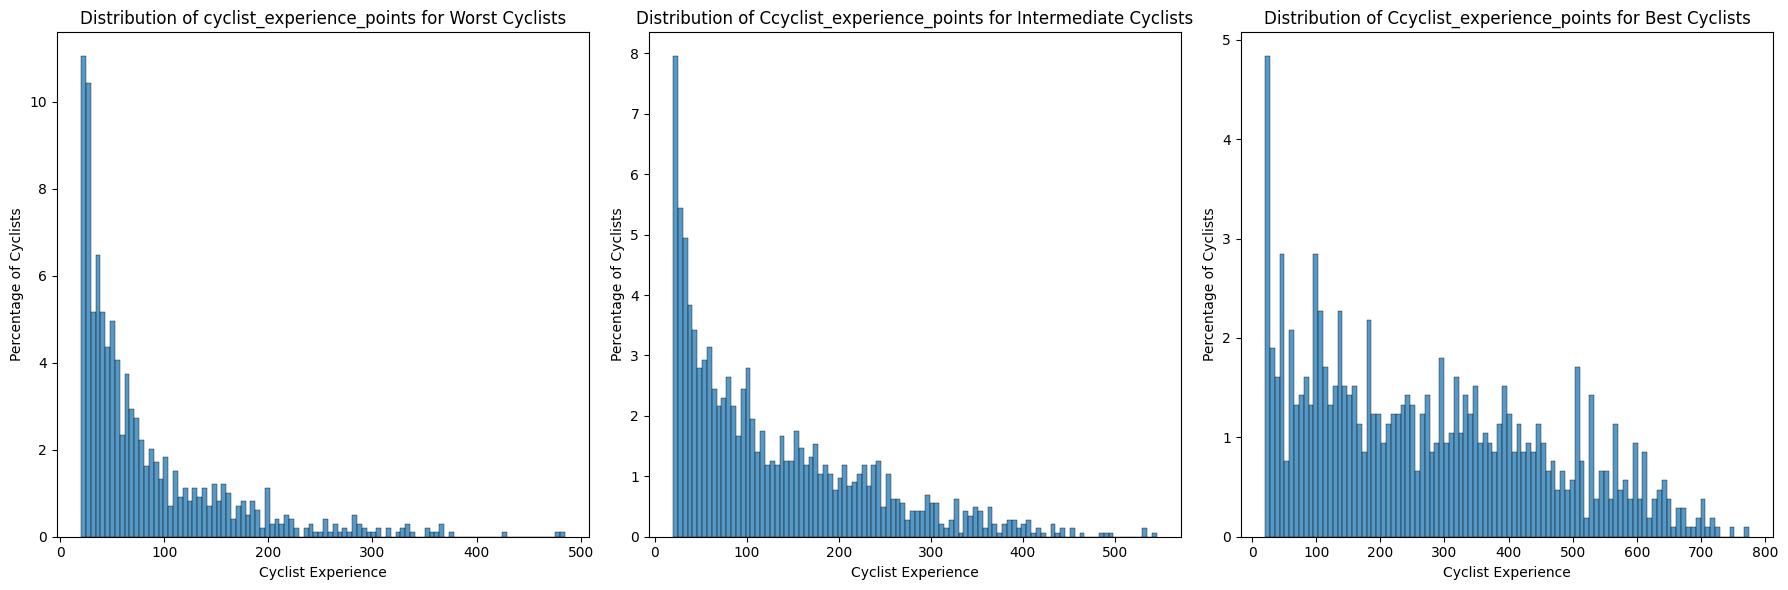
\includegraphics[width=0.93\textwidth]{images/CLUSTER/k-means/experience_distr.png}  
\caption{ \small K-means cyclist experience distribution, with cyclists represented as percentage}  
\label{fig:experience_distr_kmenas}  
\end{figure}  

\noindent  
Examining the \textbf{best position} achieved by cyclists, a clear distinction emerges across clusters. Figure \ref{fig:best_position_distr_kmeans} highlights that as we transition from the worst-performing cluster to the best, the proportion of cyclists achieving top positions increases significantly, while the percentage of those with lower rankings as best positioning decreases.  

\begin{figure}[H]  
\centering  
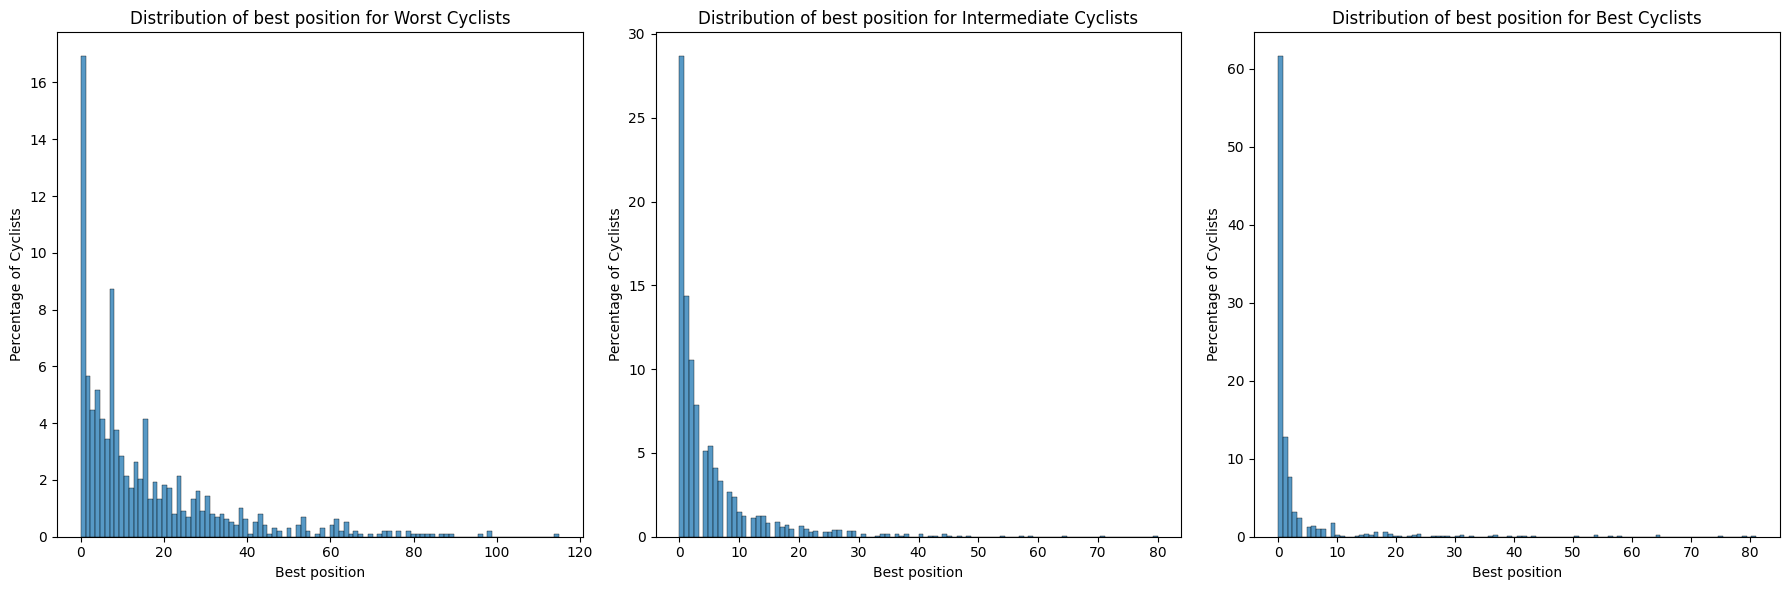
\includegraphics[width=0.93\textwidth]{images/CLUSTER/k-means/best_position_distr.png}  
\caption{ \small K-means best position distribution, with cyclists represented as percentage}  
\label{fig:best_position_distr_kmeans}  
\end{figure}  

\noindent  
\textbf{Performance entropy} shows a slight increase among higher-performing clusters, as illustrated in \autoref{fig:performance_entropy_distr_kmeans}. This result, while counterintuitive at first glance, can be explained by the larger number of races participated in by top cyclists, including high-level ones. Such extensive participation introduces variability in their results. In contrast, lower-level cyclists often compete in fewer races, leading to more consistent but less remarkable performances.  

\begin{figure}[H]  
\centering  
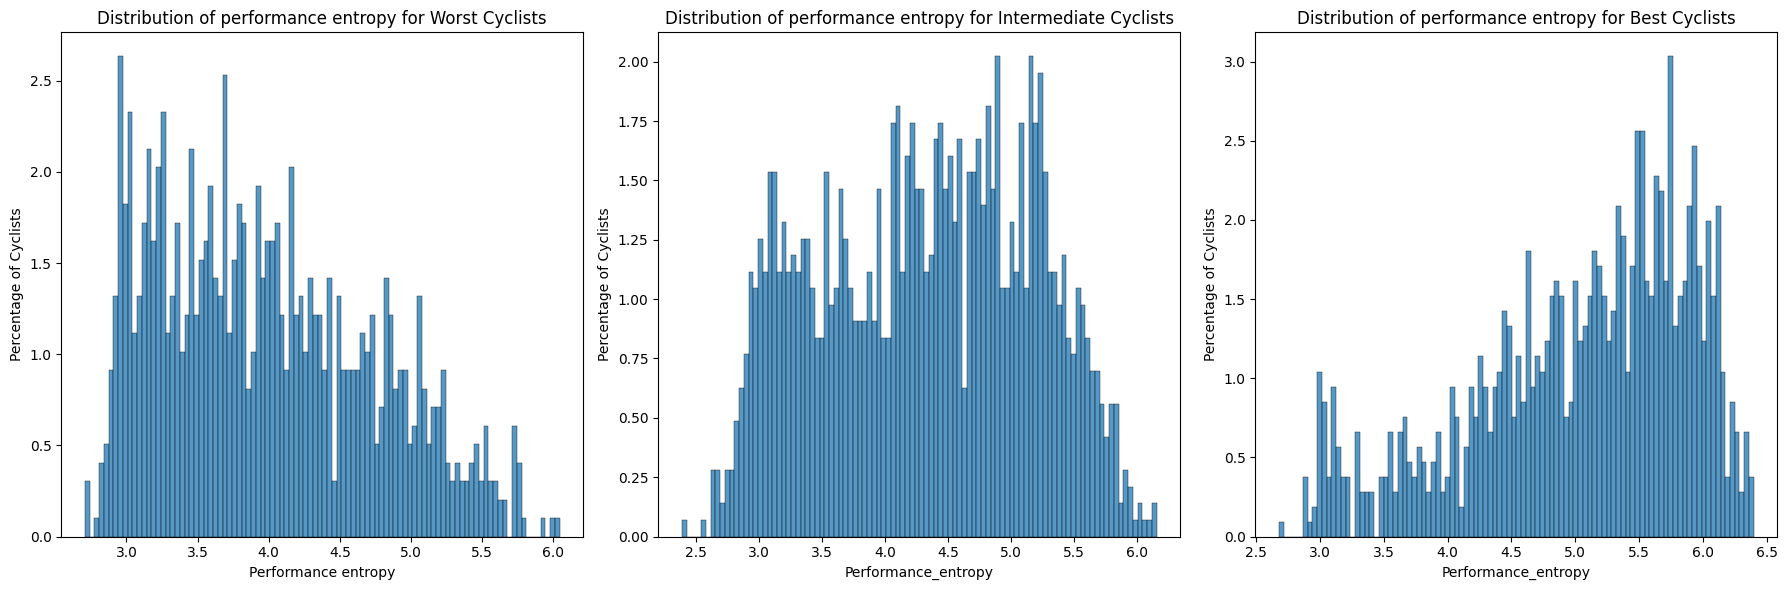
\includegraphics[width=0.93\textwidth]{images/CLUSTER/k-means/performance_entropy_distr.png}  
\caption{ \small K-means performance entropy distribution, with cyclists represented as percentage}  
\label{fig:performance_entropy_distr_kmeans}  
\end{figure}  


\noindent
\textbf{Final Analysis and Conclusions}\\
The identified clusters exhibit feature distributions that align with our expectations of a cyclist’s skill level confirming that K-means effectively groups cyclists based on their skill levels. Despite this, the distributions of extra-clustering features reveal that the classes are not perfectly separated into distinct bins. High or low values of certain features can still be observed in clusters where they would not be expected.

We can also notice that skill level is determined not only by strong race results, weighted by the importance of the competitions, but also by career activity. Incorporating the career level feature allowed the clustering to identify a "rank" that accounts for both performance and participation throughout a cyclist’s career.  

As a result, a cyclist who has competed in only a few races and won them all may not be classified among the best. This is because the career level feature factors in the total number of completed races and the cumulative score, weighted by race importance. \\

\noindent
\textbf{Summary:}    

\begin{itemize}
    \vspace{-0.20cm}
    \item \textbf{Best Cyclists cluster}: Cyclists who achieved excellent average results, with many podiums and extensive experience in high-level races.
    \vspace{-0.20cm}
    \item \textbf{Intermediate Cyclists cluster}: Cyclists with a good number of races and discrete average results, with experience in medium-level races.
    \vspace{-0.20cm}
    \item \textbf{Worst Cyclists cluster}: Cyclists who achieved generally poor results in low-level races and/or have limited experience.
\end{itemize}

We want also to highlight that another configuration of features was tested with K-means using \textit{mean\_last\_20\_position} instead of \textit{mean\_sq}. This was because we wanted to include information related to underperformance as well. The results obtained are significant, but not as optimal as those of the first feature configuration. All the details are in the notebook \texttt{TASK\_3/k\_means.ipynb}.

%---------------------------------------------------------


\subsection{X-means}
X-means provides a fairly clear separation between the clusters of worst, intermediate, and best cyclists with a slightly lower level of accuracy than K-means. In \autoref{fig:pairplot_xmeans} we can see PCA and pair plot.

\begin{figure}[H]
\centering
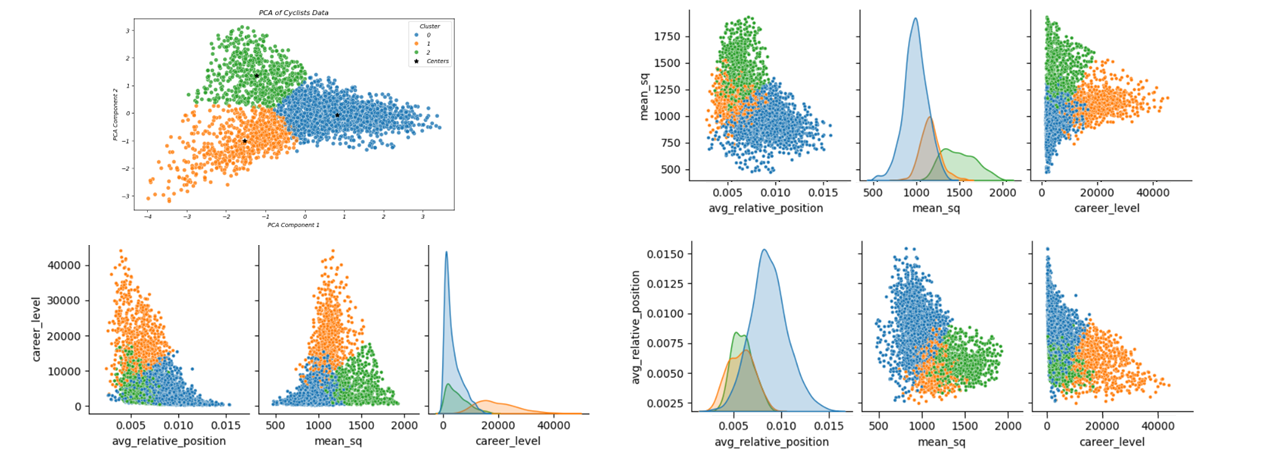
\includegraphics[width=0.93\textwidth]{images/CLUSTER/X-means/pairplot.png}
\caption{ \small  X-means feature pair plots and PCA visualization \small}
\label{fig:pairplot_xmeans}
\end{figure}

\subsubsection{Characterization}

After full characterization (the same as used for K-means), the clusters were mapped as follows: \textbf{cluster 0 = worst cyclists}, \textbf{cluster 1 = best cyclists}, and \textbf{cluster 2 = intermediate cyclists}. We can observe some key features through an initial analysis of the plot of the centroid values shown in the \autoref{fig:cluster_centroids_xmeans}.
For the intermediate cyclists cluster, the centroid value of \textit{start\_list\_quality} is significantly higher than that of the worst cyclists cluster. We can also notice that the difference in average position between intermediate and top cyclists clusters is almost negligible. In the end, the \textit{career\_level} of the intermediate cyclists cluster is very close to that of the worst cyclists cluster.\\

\noindent
The rest of the characterization yielded results similar to those of K-means, although not identical. From this, we made the following observations:
\begin{enumerate}
    \item \textbf{Worst Cyclists Cluster}: cyclists who have participated in relatively fewer races on average compared to the best cyclist cluster, achieving high (so not good) placements in low-importance races.

    \item \textbf{Best Cyclists Cluster}:  
    in this cluster, some cyclists have competed in a large number of races (which is the reason why they have a very high \textit{career\_level} value) and have achieved good placements on average slightly better than those of the cyclists in the intermediate cluster. The average start list quality is quite low compared to the intermediate cluster, which means that despite competing in many races, many of them were not always at a high level.

    \item \textbf{Cluster Intermediate Cyclists}:  
    in this cluster, some cyclists have participated in a relatively small number of races compared to the best cyclists cluster (unlike K-means, X-means shows a larger experience gap between these two clusters) but they have achieved good placements and have competed in high-level races.
\end{enumerate}

\noindent
\textbf{Summary}
\begin{itemize}
    \item \textbf{Worst Cyclists Cluster}: represents the worst cyclists in terms of experience, results, and career level.
    \item \textbf{Intermediate Cyclists Cluster}: includes cyclists with not-so-high experience but great results in high-quality races.
    \item \textbf{Best Cyclists Cluster}: includes cyclists with the best average results compared to other clusters (slightly better than the intermediates), high experience, and a high career level but a low \textit{mean\_sq} value.
\end{itemize}

\begin{figure}[H]
\centering
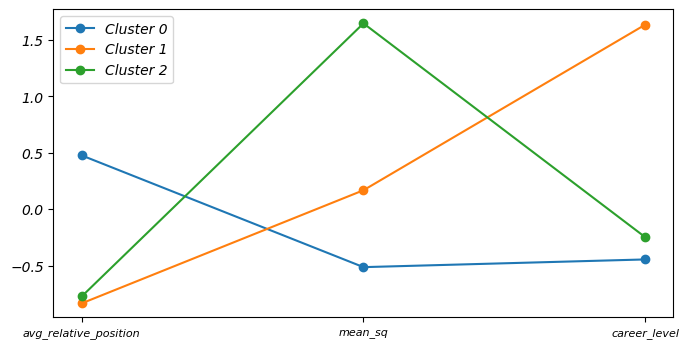
\includegraphics[width=0.5\textwidth]{images/CLUSTER/X-means/centroids_plot.png}
\caption{ \small \small Parallel Coordinates Plot for X-means Centroids}
\label{fig:cluster_centroids_xmeans}
\end{figure}

\noindent
In general, we can say that the results obtained are fairly interpretable but slightly more confusing compared to those from K-means.

%--------------------------------------------------- 
\subsection{Hierarchical Clustering}
We performed an agglomerative hierarchical clustering on the same features highlighted in the previous sections. \\

\subsubsection{Best Parameters Search}
To find a suitable configuration, we searched all possible combinations of metrics and associated methods, testing several cluster numbers of 3, 4, 5, 6, and 10 for each. Finally we calculated the silhouette and DB scores to assess them. We sorted the results by decreasing silhouette and increasing DB scores and looked at the top twenty configurations. We then explored each one by hand and found that the one that came closest to our needs used \texttt{correlation} as metric with \texttt{average} method and found 3 clusters with a 0.35 as silhouette score and 1.09 as DB score. \\

\subsubsection{Characterization}
As one can see from \autoref{fig:hier-plots} the algorithm identified three distinct clusters. The dendrogram on the left shows the hierarchical clustering of the data based on correlation distance and the average linkage method. The leftmost cluster is more separated from the other two, indicating a higher dissimilarity. The remaining two clusters are more closely grouped, suggesting that they may share similar characteristics.

\begin{figure}[H]
    \centering
    \begin{subfigure}[b]{0.33\textwidth}
        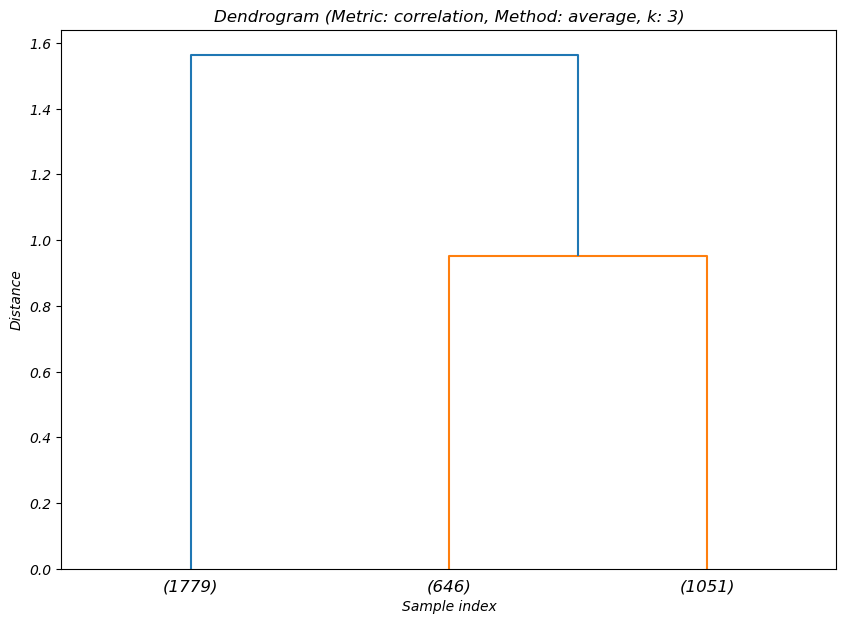
\includegraphics[width=\textwidth]{images/CLUSTER/hierarchical/dendogram.png}
    \end{subfigure}
    \begin{subfigure}[b]{0.33\textwidth}
        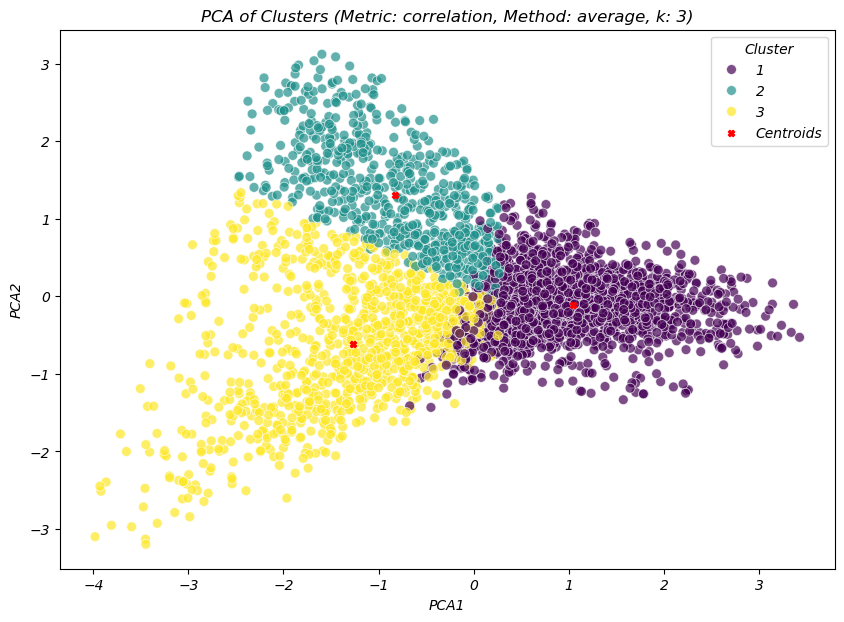
\includegraphics[width=\textwidth]{images/CLUSTER/hierarchical/pca.png}

    \end{subfigure}
    \begin{subfigure}[b]{0.5\textwidth}
        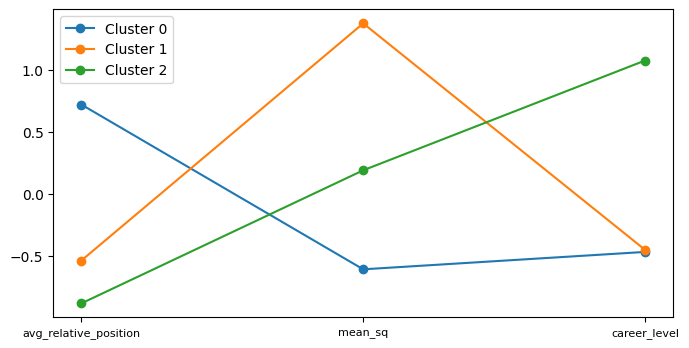
\includegraphics[width=\textwidth]{images/CLUSTER/hierarchical/coordinates_hier.png}
    \end{subfigure}
    \caption{ \small From left to right: Dendogram, 2D PCA and Parallel Coordinates Plot for hierarchical clusters computed centroids }
    \label{fig:hier-plots}
\end{figure}

\noindent From the Parallel Coordinates Plot, we hypothesized that: \textbf{Cluster 0} might group the worst cyclists (very low average relative position, a medium mean start list quality, and a very high career level, \textbf{Cluster 1} the intermediate ones (slightly higher career level than those in \textbf{Cluster 0}, but with a lower average relative position and the highest start list quality in the clustering) and finally the \textbf{Cluster 2} the best ones (very low average relative position, a medium mean start list quality, and a very high career level). Overall, results are very similar to the one obtained with X-means.

To check if our hypothesis held, we plotted the distributions of \textit{weighted\_podiums}, \\\textit{cyclist\_experience} and \textit{performance\_entropy} in each cluster found. The worst cyclists typically show low or null podiums, the best cyclists show higher feature values and intermediate cyclists fall in between, with some overlap. Although this overlap is minimal, we find the interpretation less clear than in K-Means where the subdivision was clearer. The distribution of experience is similar in the worst and intermediate clusters, but the best cyclists have much higher average experience, correlating with a higher career level. The percentage of cyclists with higher performance entropy increases slightly from the worst to the best cyclists. This is due to higher-performing cyclists participating in more races, leading to more fluctuating results. In contrast, lower-performing cyclists tend to have fewer races, resulting in more regular performance with fewer peaks. \\

\noindent\textbf{Conclusion}\\
Although the final result is the similar to K-means, we believe that K-means is better at grouping riders based on their overall performance.

\subsection{DB-Scan Clustering}
The DB-Scan clustering was the poorest one in terms of result quality. The following sections describe the process.\\

\noindent\textbf{Best Parameters Search}\\
To optimize the clustering process, we started constructing the distance matrix for the scaled dataset and identifying the 5 nearest neighbors for each data point. Leveraging the Kneedle library for the elbow method, we found the critical elbow in the sorted distance curve. We then tested different values for \texttt{min\_samples} (5, 7, 10, 12, 15, 20, 25, 30, 50, 80) and \texttt{epsilon}, selecting 200 linearly spaced values between 0.01 and 1. The best DBSCAN fit found only one cluster with all the data, which wasn't surprising given the data's lack of dense, disconnected structures. In a second trial, after analyzing results with more than one cluster, the best result came from \texttt{min\_samples} = 12 and \texttt{eps} = 0.065, yielding 2 clusters and outliers. However, as observed in \autoref{fig:dbscan-pca}, the results were not promising.

\begin{figure}[h]
    \centering
    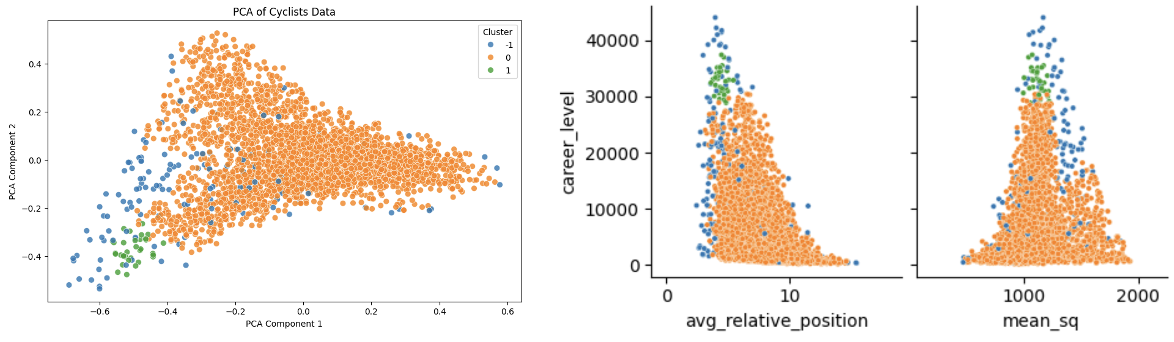
\includegraphics[width=0.8\linewidth]{images/CLUSTER/dbscan/pca.png}
    \caption{ \small DBSCAN Pairlplot and PCA}
    \label{fig:dbscan-pca}
\end{figure}

\noindent We found that cyclists in \textbf{Cluster 1} (the best cluster) had won at least one stage, while most in \textbf{Cluster 0} had not. Surprisingly, 75\% of the cyclists in the outlier cluster won at least one stage, suggesting outliers may be high-performance cyclists. This cluster also includes cyclists with both high and low experience levels. Top cyclists show higher performance variability, likely due to their greater experience and participation in more stages. When considering career levels, \textbf{Cluster 1} represents the best cyclists, though some are in \textbf{Cluster 0}'s tail and many in the outliers cluster, which also contains cyclists with low experience and career levels due to the distribution of professionals.\\

\noindent\textbf{Conclusion}\\
Overall, \textbf{Cluster 1} contains cyclists with higher career levels, more experience, and more wins, along with better race positions and greater variability. These cyclists' superior performance is linked to extensive racing experience. The \textbf{Cluster 0} tries to group the rest. We think that the clustering quality does not match K-Means.

\subsection{Comparison of metrics}
From Table \ref{tab:clustering_results}, we can observe that K-means and X-means achieve the best results, with the lowest Davies-Bouldin scores and highest Silhouette scores, indicating well-separated and compact clusters. These findings align with their strong performance during cluster characterization.

While X-means slightly outperforms K-means in compactness and separation, K-means offers greater clarity and precision in cluster characterization.

\begin{table}[H]
    \centering
    \scriptsize
    \begin{tabular}{p{2.0cm}ccccccc}
    \toprule
    \textbf{Model} & \textbf{SSE} & \textbf{Silhouette} & \textbf{Davies-Bouldin Score} \\
    \midrule
    \textbf{K-means} 
      & 4468
      & 0.40
      & 0.93 \\
    \textbf{X-means} 
      & 4535
      & 0.41
      & 0.86 \\
    \textbf{DBSCAN} 
      & -
      & 0.29
      & 1.54\\
    \textbf{Hierarchical} 
      & -
      & 0.35
      & 1.09 \\
    \bottomrule
    \end{tabular}
    \caption{ \small \small Cluster Algorithm Metrics Comparison}
    \label{tab:clustering_results}
\end{table}